\chapter{Proposed Solution}

\graphicspath{{contribution/figures/}}

In this chapter, we delve into the implementation details of our proposed solution, designed to enhance the efficiency and accuracy of information retrieval through a Local Retrieval-Augmented Generation (RAG) agent. Our solution leverages a variety of advanced technologies, including FastAPI\footnote{\url{https://fastapi.tiangolo.com/}}, Langchain\footnote{\url{https://python.langchain.com/v0.1/docs/get_started/introduction}}, Langraph\footnote{\url{https://python.langchain.com/v0.1/docs/langgraph/}}, Ollama\footnote{\url{https://www.ollama.com/}}, Docker, Docker Compose\footnote{\url{https://www.docker.com/}}, and LangSmith\footnote{\url{https://www.langchain.com/langsmith}}. By integrating these tools, our aim is to create a robust, scalable, and efficient system capable of serving both local and web-based information needs.

Our implementation focuses exclusively on using LLaMA3 for the language model component. This approach ensures that we can thoroughly evaluate and optimize the performance of LLaMA3 in the context of our application.

We will begin by discussing the high-level architecture of our solution, highlighting the key components and their interactions. This will be followed by an overview of the backend implementation, which leverages FastAPI, Langchain, and Langraph for efficient document retrieval and model serving, complemented by Ollama for local model serving. We will also cover the use of Docker and Docker Compose for containerization and deployment, ensuring the scalability and reliability of our backend services. Additionally, we will discuss the integration of LangSmith for tracing and logging LLM outputs to monitor and improve system performance.

Throughout this chapter, we will provide a comprehensive overview of the data flow, from the initial user query to the final generated answer, elucidating the intricacies of our system's workflow. Finally, we will address the challenges encountered and the solutions devised to overcome them.

\section{Problem Definition}

In the era of rapid information growth and increasing complexity of queries, traditional question-answering systems often struggle to provide comprehensive and accurate responses. These systems frequently rely on a single approach, such as keyword-based retrieval or language model generation, which can lead to suboptimal results. Furthermore, many existing systems are limited to a predefined knowledge base or corpus, restricting their ability to adapt and incorporate the latest information from the vast expanse of the internet.

Traditional question-answering approaches may also suffer from issues such as hallucinations \cite{zhang2023sirens} or failing to address the core aspects of a query. There is a need for a more advanced and adaptive question-answering system that can leverage the strengths of various retrieval and generation techniques, while also accounting for potential limitations or errors.

The goal of our project is to develop a Local RAG (Retrieval-Augmented Generation) agent with LLaMA3 and other open source LLMs that combines ideas from several state-of-the-art RAG papers. This agent aims to provide more accurate and comprehensive answers to a wide range of queries by intelligently routing queries, utilizing fallback mechanisms, and incorporating self-correction capabilities. The Local RAG agent will leverage the power of large language models like LLaMA3, while also incorporating retrieval techniques to ground the responses in relevant information sources. Additionally, the agent will have the ability to fall back to web search when the available information is insufficient, and self-correct its responses to address potential hallucinations or incomplete answers.

By combining these different approaches, the Local RAG agent aims to overcome the limitations of traditional question-answering systems, providing users with more reliable, up-to-date, and context-aware responses.

\section{Solution Overview}

\begin{figure}[!ht]
    \centering
    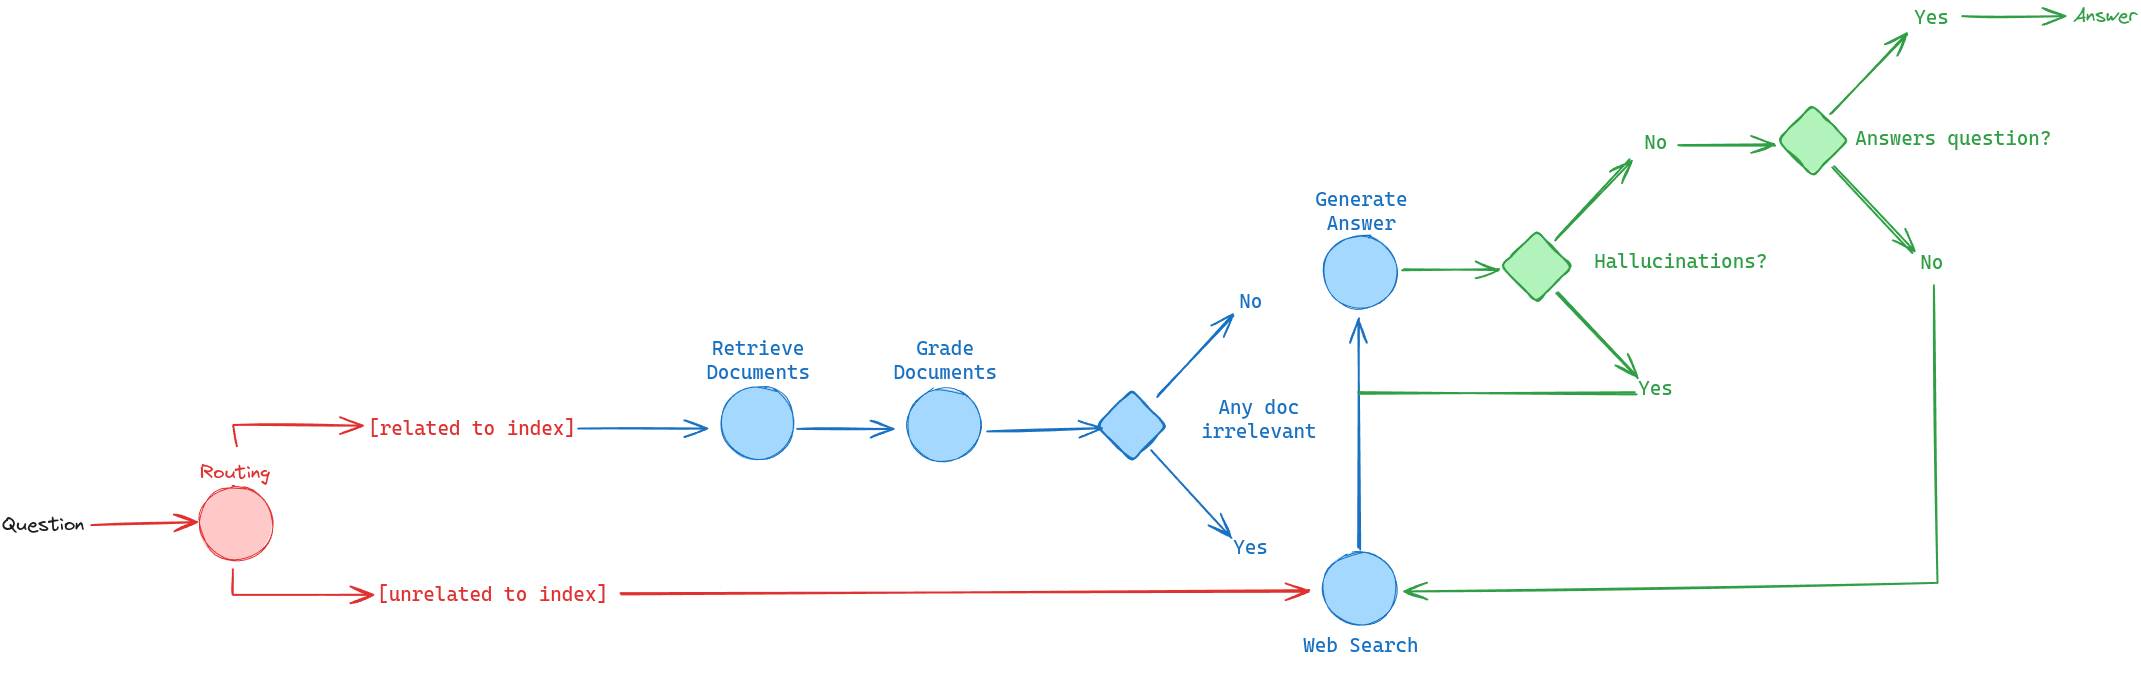
\includegraphics[width=\linewidth]{architecture.png}
    \caption{\it{Proposed solution architecture.}}
\end{figure}

\subsection{High-Level Architecture}

Our solution aims to develop a Local Retrieval-Augmented Generation (RAG) agent using LLaMA3. The architecture is designed to efficiently manage the entire process of information retrieval and answer generation. Below, we outline the primary components and their interactions:

\begin{enumerate}
    \item \textbf{User Query Input:} Users submit queries to the system through an API endpoint.

    \item \textbf{Routing:} The system routes the incoming queries to appropriate retrieval approaches using a routing mechanism. Queries that are relevant to the indexed documents are processed through the local retrieval system. Queries that are not relevant to the indexed documents are routed to a fallback mechanism for web search.

    \item \textbf{Document Retrieval and Grading:} The retrieval system fetches relevant documents from the index. Retrieved documents are graded based on relevance and quality using Langchain and Langraph.

    \item \textbf{Model Serving with Ollama:} LLaMA3 models are served locally using Ollama. The system uses these models to generate answers based on the retrieved and graded documents.

    \item \textbf{Answer Generation and Validation:} Generated answers are validated for relevance and accuracy. The system checks for hallucinations and ensures the answer addresses the user's query.

    \item \textbf{Fallback to Web Search:} If the retrieved documents are not relevant, the system falls back to a web search. This ensures that users receive comprehensive answers even if the local index does not have relevant information.

    \item \textbf{Self-Correction and Final Answer:} The system self-corrects any answers with hallucinations or that do not address the question properly. The final validated answer is returned to the user.

    \item \textbf{Logging and Monitoring with LangSmith:} LangSmith is integrated to trace and log the outputs of the LLM. This allows monitoring and improving the performance of the system.

\end{enumerate}

\subsection{Key Technologies and Frameworks}

\begin{itemize}
    \item \textbf{FastAPI:} Chosen for its high performance and ease of use in building robust APIs. Facilitates the development of a scalable and efficient backend system.

    \item \textbf{Langchain and Langraph:} Used for document retrieval and grading. These frameworks help in efficiently managing and processing large volumes of text data.

    \item \textbf{ChromaDB:} Utilized as the vector database for efficient document retrieval. Enhances the retrieval process by providing fast and accurate vector search capabilities.

    \item \textbf{Ollama:} Responsible for serving LLaMA3 models locally. Ensures efficient model management and minimizes latency.

    \item \textbf{Docker and Docker Compose:} Used for containerizing backend services. Ensures consistency across different environments and simplifies deployment.

    \item \textbf{LangSmith:} Integrated for tracing and logging LLM outputs. Enhances monitoring capabilities and aids in performance optimization.
\end{itemize}

\subsection{Data Flow}

\begin{enumerate}
    \item \textbf{Query Reception:} The user submits a query to the FastAPI endpoint. The query is routed based on its relevance to the indexed documents.

    \item \textbf{Document Processing:} Relevant documents are retrieved from ChromaDB and graded. Irrelevant queries are redirected to a fallback web search.

    \item \textbf{Model Interaction:} The system interacts with LLaMA3 models through Ollama to generate answers. LangSmith monitors and logs these interactions for performance tracking.

    \item \textbf{Answer Validation:} Generated answers are validated and corrected if necessary. The final answer is then delivered to the user.
\end{enumerate}

\section{Detailed Workflow}

The workflow of our Local Retrieval-Augmented Generation (RAG) agent involves several key steps, from the initial query submission to the final generation and validation of answers. Here, we delve into each step to provide a comprehensive understanding of the process.

\subsection{Question Routing}

\begin{figure}[H]
    \centering
    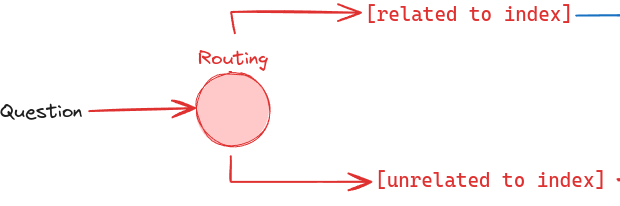
\includegraphics[width=\textwidth,height=6cm,keepaspectratio=true]{routing.png}
    \caption{
        \it{Question Routing}
    }
\end{figure}

The workflow begins with the user submitting a query via a FastAPI endpoint. This endpoint is designed to handle incoming requests efficiently and forward them to the appropriate processing unit. Upon receiving a query, the system evaluates its relevance to the indexed documents. This evaluation determines whether the query can be answered using the locally stored documents or if it needs to be redirected to a fallback mechanism that utilizes web search.

For queries that are relevant to the indexed content, the system routes them to the local retrieval system. If the query is deemed unrelated to the indexed content, the system redirects it to the fallback mechanism, ensuring that users receive comprehensive answers even if the local index does not contain relevant information.

\subsection{Document Retrieval and Grading}

\begin{figure}[H]
    \centering
    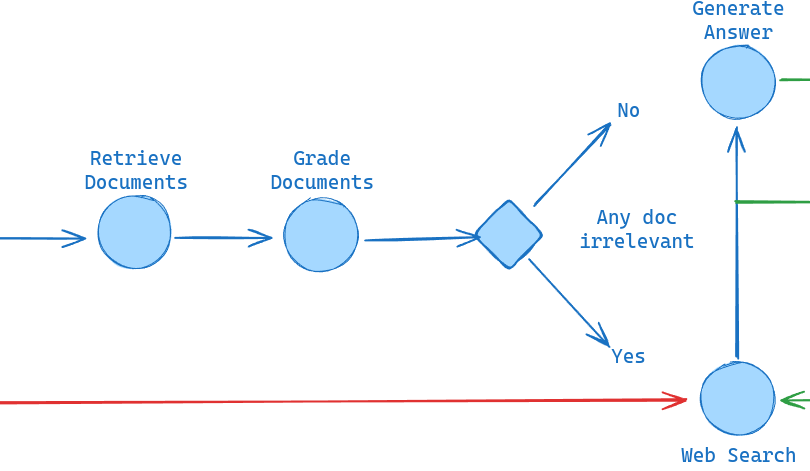
\includegraphics[width=\textwidth,height=6cm,keepaspectratio=true]{retrieval.png}
    \caption{
        \it{Document Retrieval and Grading}
    }
\end{figure}

For queries routed to the local retrieval system, the next step is to fetch relevant documents from the ChromaDB vector database. ChromaDB employs vector search techniques to find the most relevant documents based on the query vector. This process involves converting the query into a vector representation and searching the database for documents with similar vector representations.

Once the relevant documents are retrieved, they undergo a grading process using the LLaMA3 model. The model evaluates the relevance and quality of the retrieved documents, ensuring that only the most pertinent documents are used for answer generation. This grading process is essential to maintain the quality and relevance of the information provided to the user.

If any document is found irrelevant during the grading process, the system flags it and prepares to use the fallback web search mechanism. This step is crucial to maintain the quality and relevance of the information provided to the user.

\subsection{Model Interaction with Ollama}

\begin{figure}[H]
    \centering
    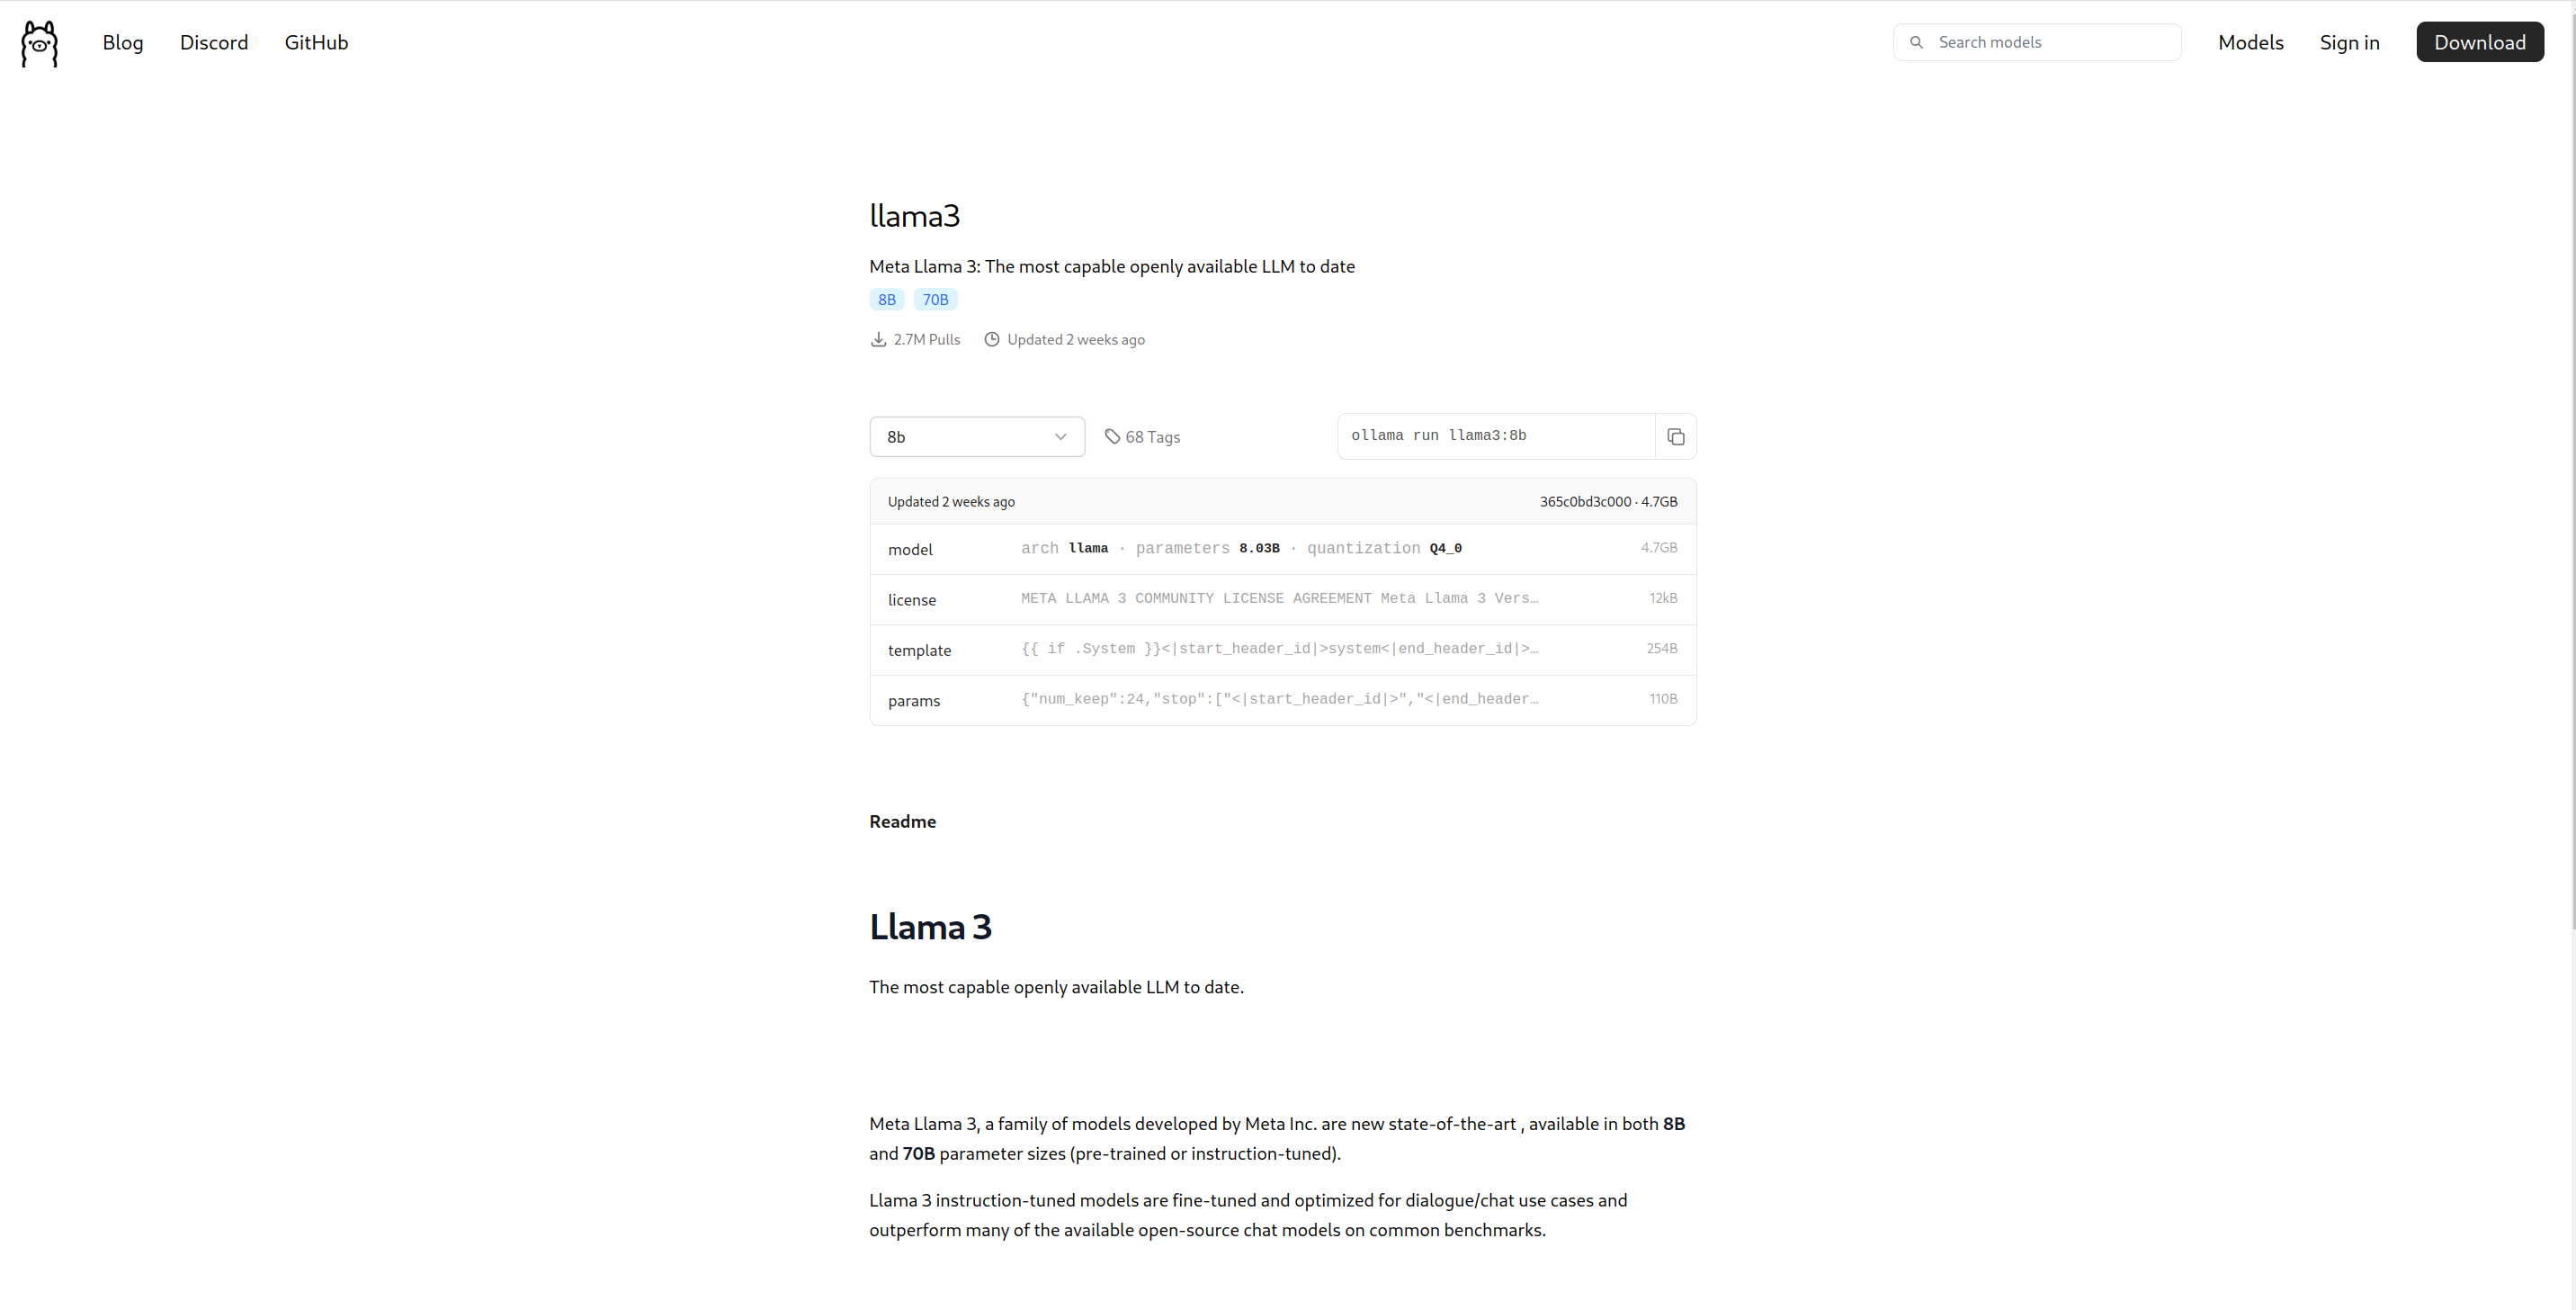
\includegraphics[width=\textwidth,height=6cm,keepaspectratio=true]{ollama.png}
    \caption{
        \it{Llama3's page on ollama website.}
    }
\end{figure}

With the relevant and graded documents in hand, the system then interacts with the LLaMA3 models served locally using Ollama. Ollama ensures low-latency and efficient model interaction by managing the lifecycle of the models and ensuring they are readily available for processing incoming queries.

The LLaMA3 model takes the query and the graded documents as input to generate a coherent and relevant answer. This model interaction is critical as it synthesizes the information from the documents and produces a response tailored to the user's query. By using locally served models, the system minimizes latency and enhances performance, providing users with quick and accurate responses.

\subsection{Answer Validation and Correction}

\begin{figure}[H]
    \centering
    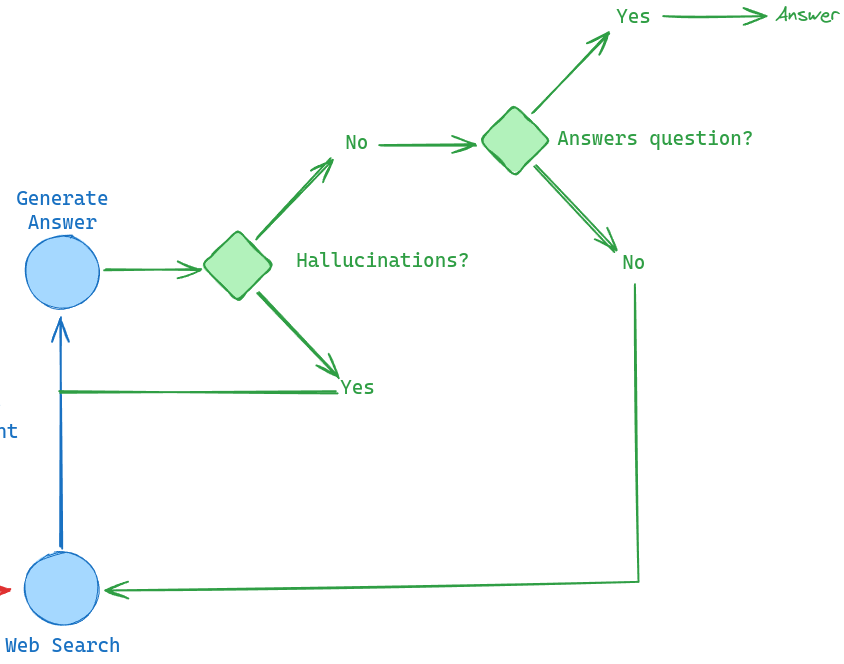
\includegraphics[width=\textwidth,height=6cm,keepaspectratio=true]{correction.png}
    \caption{
        \it{Answer validation and correction.}
    }
\end{figure}

Once an answer is generated, it undergoes an initial validation process to check for relevance and accuracy. The system evaluates whether the answer sufficiently addresses the user's query and ensures it is free from hallucinations—instances where the model generates incorrect or nonsensical information.

If hallucinations or other issues are detected, the answer is flagged for further correction. The system includes a self-correction mechanism that refines answers with detected issues. This mechanism leverages additional passes through the model and grading processes to improve the answer quality. If the initial validation fails or if the retrieved documents were not relevant, the system employs the fallback mechanism to perform a web search. The results from the web search are then processed and used to generate a new answer.

After any necessary corrections, the answer undergoes a final validation step to ensure it is accurate, relevant, and free from hallucinations. This step is crucial to maintain the integrity and reliability of the system's responses.

\subsection{Final Answer Delivery}

Once the answer has been validated and corrected, it is ready for delivery. The final validated answer is sent back to the user through the FastAPI endpoint. This endpoint handles the response and ensures that the user receives a comprehensive and accurate answer to their query.

The user interaction ends here, but the system continues to monitor and log the entire process to improve future responses. By maintaining a high standard of validation and correction, the system ensures that users consistently receive high-quality information.

\subsection{Logging and Monitoring with LangSmith}

\begin{figure}[H]
    \centering
    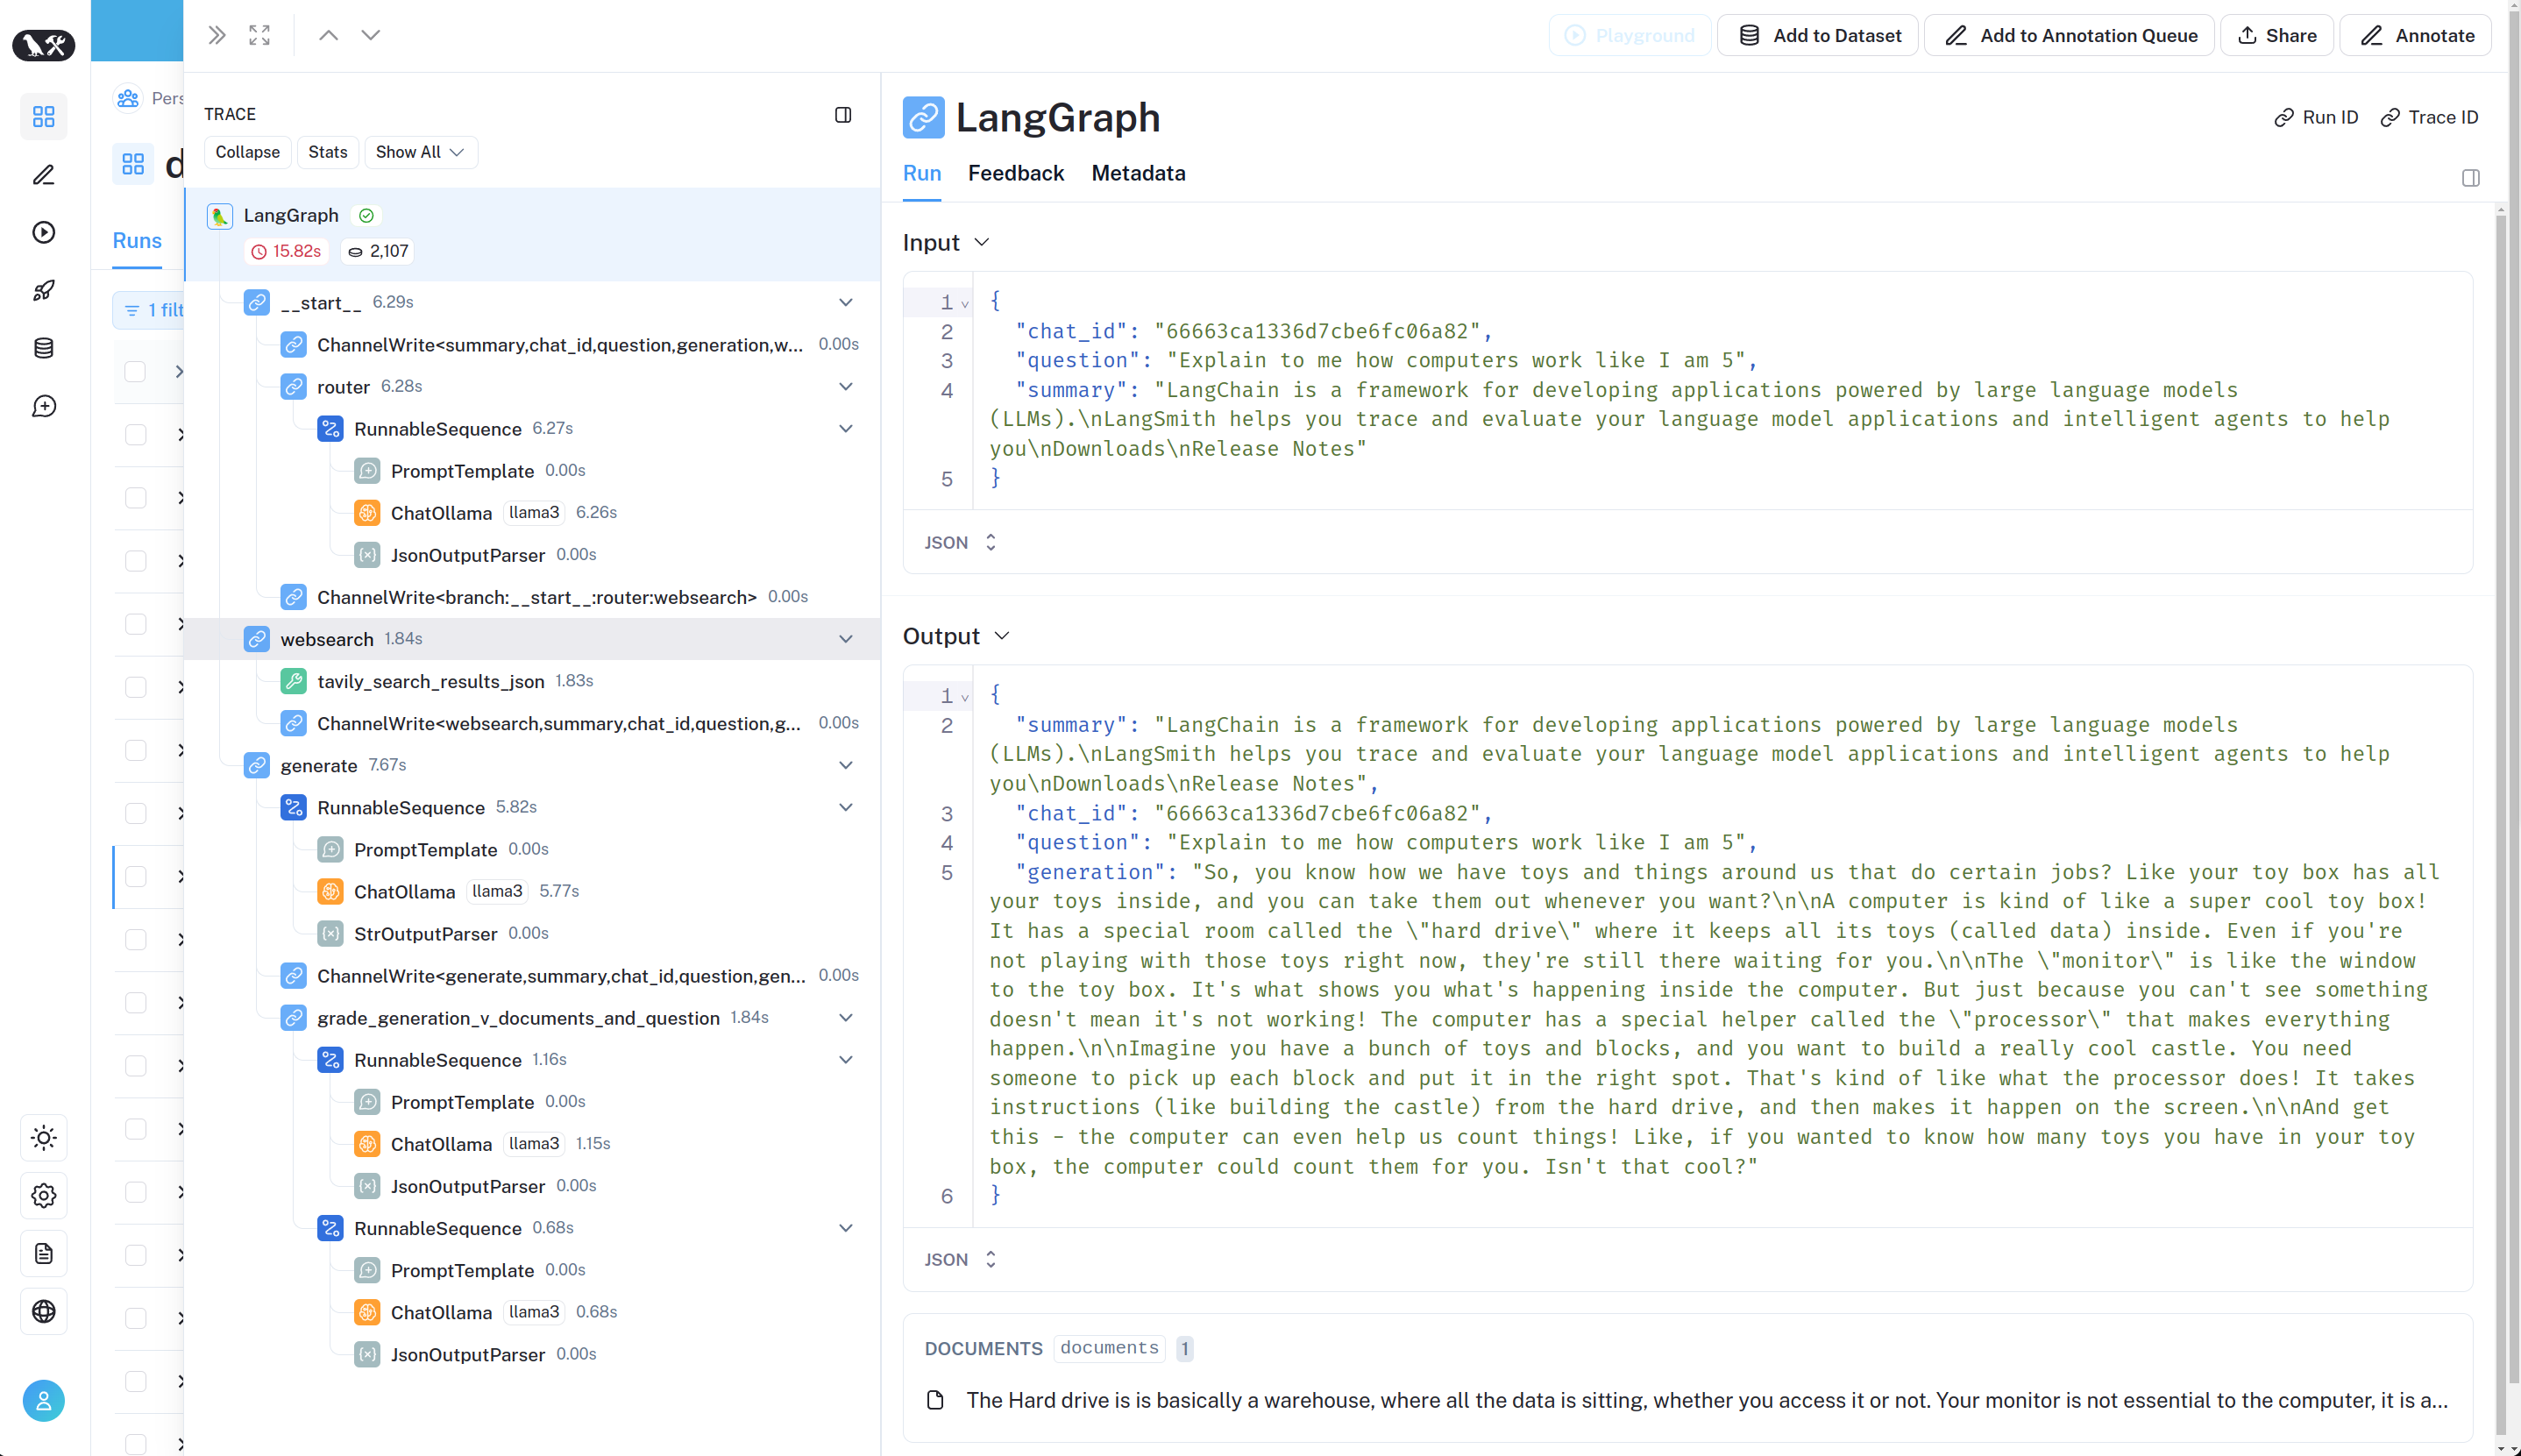
\includegraphics[width=\textwidth,height=6cm,keepaspectratio=true]{langsmith.png}
    \caption{
        \it{Logging and Monitoring with LangSmith.}
    }
\end{figure}

Throughout the entire workflow, LangSmith is used to trace and log the outputs of the LLM. This includes logging the initial query, the retrieved documents, the generated answers, and any corrections made. LangSmith provides tools to monitor the performance of the system, identifying bottlenecks and areas for improvement.

This continuous monitoring and logging are crucial for maintaining the system's performance and reliability. By analyzing the logs, we can pinpoint issues and optimize the system to handle future queries more efficiently. LangSmith's integration enhances the system's ability to provide accurate and relevant responses while also allowing for continuous improvement.

\section{Challenges and Solutions}

Developing and implementing a Local Retrieval-Augmented Generation (RAG) agent using LLaMA3 involves several challenges, from integrating various technologies to ensuring the system's performance and reliability. Below, we discuss some of the key challenges encountered during the development process and the solutions implemented to address them.

\subsection{Integration of Diverse Technologies}

\textbf{Challenge:} Integrating multiple technologies such as FastAPI, Langchain, ChromaDB, Ollama, and LangSmith can be complex and time-consuming. Ensuring that these components work seamlessly together is critical for the overall performance of the system.

\textbf{Solution:} To address this challenge, a modular architecture was adopted, where each component is designed as an independent module with well-defined interfaces. Docker and Docker Compose were used to containerize each service, ensuring consistency across different environments. This modular approach simplifies the integration process and makes it easier to isolate and troubleshoot issues. Comprehensive integration testing was conducted to ensure that all components work together as expected.

\subsection{Efficient Document Retrieval}

\textbf{Challenge:} Efficiently retrieving relevant documents from a large dataset using vector search can be computationally intensive and time-consuming, potentially leading to latency issues.

\textbf{Solution:} ChromaDB was chosen as the vector database due to its optimized vector search capabilities. The system leverages advanced indexing and search algorithms to quickly retrieve the most relevant documents.

\subsection{Document Grading Accuracy}

\textbf{Challenge:} Ensuring the accuracy of document grading is crucial for generating high-quality answers. Incorrectly graded documents can lead to irrelevant or inaccurate answers.

\textbf{Solution:} The LLaMA3 model was utilized for both document grading and answer generation. By employing prompting techniques, the LLaMA3 model evaluates the relevance and quality of the retrieved documents, ensuring that only the most pertinent documents are used for answer generation. This approach maintains consistency and leverages the model's inherent capabilities without the need for fine-tuning.

\subsection{Monitoring and Logging}

\textbf{Challenge:} Monitoring the performance and behavior of the system in real-time, and logging all interactions to identify and troubleshoot issues, is crucial for maintaining reliability.

\textbf{Solution:} LangSmith was integrated into the system to provide comprehensive logging and monitoring capabilities. LangSmith traces and logs every interaction, from the initial query to the final answer delivery. These logs are analyzed to identify performance bottlenecks and areas for improvement. Real-time monitoring dashboards were set up to track key performance metrics, allowing for proactive maintenance and optimization of the system.

\section{Conclusion}

In conclusion, the implementation of this Local Retrieval-Augmented Generation agent demonstrates a comprehensive approach to leveraging state-of-the-art technologies for efficient and accurate information retrieval and generation. By addressing key challenges with targeted solutions, we created a scalable and robust system capable of providing high-quality responses to user queries. The continuous monitoring and logging with LangSmith ensure that the system can be maintained and optimized over time, ensuring sustained performance and reliability.